% !TEX root = pfe-book2.tex
%!TEX TS-program = pdflatex
%!TEX encoding = UTF-8 Unicode


\cleardoublepage
%\mainmatter
\chapter{States of Matter}
\label{ch-04}


\section{Iron Vapour and Solid Air}

A strange combination of words, isn’t it? However, this is by no means nonsense: iron vapour and solid air exist in nature, only not under ordinary conditions.

But what conditions are we talking about? The state of a substance is determined by two circumstances: tem­perature and pressure.

Our lives proceed under conditions which change rela­tively little. The air pressure varies by several percent about a value of one atmosphere; the temperature of the air, say, near Moscow, lies in the interval from $-30$ to \SI{+30}{\celsius}; in the absolute scale, in which the lowest pos­sible temperature ( \SI{-273}{\celsius}) is taken as zero, this interval will look less impressive: 240-300 \si{\kelvin}, which is also only $\pm$10\% of the average value.

It is quite natural that we have become accustomed to these ordinary conditions, and so when speaking simple truths such as ``iron is a solid, air is a gas'', we forget to add ``under standard conditions''.

If iron is heated, it will first melt and then vaporize. If air is cooled, it will first liquefy and then solidify.

Even if the reader has never come across iron vapour or solid air, he or she will probably believe without difficulty that by means of a change in temperature it is possible to obtain any substance in a solid, liquid and gaseous state or, as is also said, in a solid, liquid or gaseous phase.

It is easy to believe this because everyone has observed a substance without which life on the Earth would be impossible, and that substance is in the form of a gas, a liquid, or a solid. We are speaking, of course, of water.

But under what conditions does a transformation of a substance from one state to another occur?

\section{Boiling}

If we lower a thermometer into water which has been poured into a tea-kettle, turn on the electric stove and watch the mercury in the thermometer, we shall see the following: the level of the mercury will inch upwards almost immediately. Now it is already 90, 95 and finally \SI{100}{\celsius}. The water begins boiling and simultaneously the mercury stops rising. The water has already been boiling for many minutes, but the level of the mercury does not change. The temperature will not change until all the water has boiled away (\figr{fig-4.1}).

\begin{figure}[!ht]
\centering
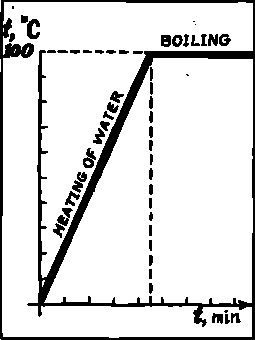
\includegraphics[width=0.4\textwidth]{figures/fig-04-01.pdf}
\caption{Temperature stays constant at boiling.}
\label{fig-4.1}
\end{figure}

But what is the heat used for if the temperature of the water does not change? The answer is obvious. The process of transforming water into steam requires energy.

Let us compare the energy of a gram of water and a gram of the steam created out of it. The molecules of the steam are distributed farther from each other than the water molecules. It is obvious that because of this the potential energy of the water will differ from that of the steam.

The potential energy of attracting particles decreases as they approach. The energy of the steam is therefore greater than that of the water, and so the transformation of water into steam requires energy. This excess energy is imparted by the electric stove to the water boiling in the tea-kettle.

The energy needed for transforming water into steam is called its \emph{heat of vaporization}. In order to transform \SI{1}{\gram} of water into steam, 539 calories are required (this figure is for a temperature of \SI{100}{\celsius}). If 539 calories are used for \SI{1}{\gram}, then $18 \times 539 \approx 9700$ calories will be supplied to 1 mole of water. This amount of heat must be consumed in breaking the intermolecular bonds. One can compare this figure with the amount of work necessary for breaking the intramolecular bonds. In order to split one mole of steam into atoms, about 220 000 calories are required, i.e. 25 times as much energy. This directly proves the weakness of the forces binding molecules to each other, as compared to the forces finding atoms together in a mole­cule.

\section{Dependence of Boiling Point on Pressure}
The boiling point of water is equal to \SI{100}{\celsius}; one might think that this is an inherent property of water, that water will always boil at \SI{100}{\celsius}, no matter where and under what conditions it may be.

But this is not so, and people who live high up in the mountains are perfectly well aware of this.

There is a tourist cabin and a scientific station near the top of Mt. Elbrus. Novices are sometimes amazed at ``how hard it is to boil an egg in boiling water'' or wonder ``why boiling water doesn’t scald.'' In such cases, it is pointed out to them that water is already boiling at \SI{82}{\celsius} on the top of Mt. Elbrus.

But what causes this? What physical factor interferes with boiling? And does the height above sea level have any significance?

This physical factor is the pressure acting on the surface of the liquid. It isn’t necessary to climb to the top of a mountain in order to check the validity of what we have said.

If we place a bell glass over water that is being heated and pump air into or out of it, we can convince ourselves that the boiling point is raised by an increase in pressure and lowered by a decrease in pressure.

Water boils at \SI{100}{\celsius} only at a definite pressure -- \SI{760}{\milli\meter\mercury} (or \SI{1}{\atmos}).

The curve showing the dependence of the boiling point on the pressure is depicted in \figr{fig-4.2}. The pressure is equal to  \SI{0.5}{\atmos} on the top of Mt. Elbrus, and a boiling point of \SI{82}{\celsius} corresponds to this pressure.

\begin{figure}[!ht]
\centering
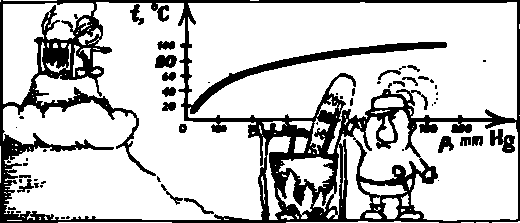
\includegraphics[width=\textwidth]{figures/fig-04-02.pdf}
\caption{Change in boiling point as a function of pressure.}
\label{fig-4.2}
\end{figure}

But it is even possible to refresh oneself in hot weather with water boiling at 10-15 \si{\milli\meter\mercury}. At such pressures, the boiling point will fall to 10-15 \si{\celsius}.

One can even obtain ``boiling water'' having a temper­ature of freezing water. One has to lower the pressure to \SI{4.6}{\milli\meter\mercury} for this.

It is possible to observe an interesting scene by placing an uncovered vessel with water under a bell glass and pumping the air out. This will make the water boil, but boiling requires heat. But since there is no air, the water has to give up its own energy. The temperature of the boiling water starts falling, but since the pumping con­tinues, the pressure also falls. Therefore, the boiling will not cease, the water will continue cooling off and will finally freeze.

Such a boiling of cold water occurs not only as a result of air being pumped out. For example, when a marine screw propeller rotates, the pressure in the layer of water moving rapidly about the metallic surface will fall sharp­ly, and so the water in this layer will boil, i.e. many bubbles filled with steam will appear in it. This phe­nomenon is called \emph{cavitation} (from the Latin \emph{cavus} meaning ``hollow'').

Decreasing the pressure, we lower the boiling point. And raising it? A graph analogous to ours answers this question. A pressure of \SI{15}{\atmos} can so delay boiling of water that it will begin only at \SI{200}{\celsius}, while a pressure of \SI{80}{\atmos} will make water boil only at \SI{300}{\celsius}.

Thus, a definite boiling point correspond to a definite external pressure. But we may also turn this assertion ``around'' by saying that ``a definite pressure corresponds to each boiling point of water''. This pressure is called the \emph{vapour pressure}.

The curve depicting the dependence of the boiling point on the pressure is simultaneously the curve of the vapour pressure as a function of the temperature.

The numbers plotted on the boiling point graph (or on the vapour pressure graph) show that the vapour pressure changes very sharply with a change in the temperature. At \SI{0}{\celsius} (i.e. \SI{273}{\kelvin}) the vapour pressure is equal to \SI{4.6}{\milli\meter\mercury}, at \SI{100}{\celsius} (\SI{373}{\kelvin}) it equals \SI{760}{\milli\meter\mercury}, i.e. has increased by a factor of 165. With a doubling of the temperature from \SI{0}{\celsius} (i.e. \SI{273}{\kelvin}) to \SI{273}{\celsius} (i.e. \SI{546}{\kelvin}), the vapour pressure grows from \SI{4.6}{\milli\meter\mercury}  to almost \SI{60}{\atmos}, i.e. by a factor of about \num{10000}.

Therefore, the boiling point, on the contrary, changes rather slowly with a change in the pressure. When the pressure is doubled, from 0.5 to \SI{1}{\atmos}, the boiling point grows from \SI{82}{\celsius} (i.e. \SI{355}{\kelvin}) to \SI{100}{\celsius} (i.e. \SI{373}{\kelvin}), and with a doubling from 1 to \SI{2}{\atmos}, from \SI{100}{\celsius} (i.e. \SI{373}{\kelvin}) to \SI{120}{\celsius} (i.e. \SI{393}{\kelvin}).

The same curve that we are now considering also con­trols the condensation of steam into water.

Steam can be transformed into water by either compress­ing or cooling it.

During the course of condensation, just as for boiling, the point will not move off the curve until the transfor­mation of steam into water or water into steam is com­pletely finished. This can also be formulated as follows: the coexistence of the liquid and the vapour phase is pos­sible under the conditions of our curve and only under these conditions. If, moreover, no heat is supplied or removed, the amount of vapour and liquid in a closed vessel will remain constant. We say that such a vapour and liquid are in equilibrium, and a vapour in equilibrium with its liquid is called saturated.

The boiling and condensation curve has, as we see, yet another meaning -- it is the curve of the equilibrium of liquid and vapour. The equilibrium curve divides the plane of the diagram into two parts. To the left and above the curve (towards higher temperatures and lower pres­sures) is the stable-vapour region. To the right and below the curve is the stable-liquid region.

The vapour-liquid equilibrium curve, i.e. the curve of the dependence of the boiling point on the pressure, or, what is the same thing, of the vapour pressure on the temperature, is approximately identical for all liquids. In some cases, the change may be somewhat sharper, in others somewhat slower, but the vapour pressure always grows rapidly with rise in temperature.

We have already used the words ``gas'' and ``vapour'' many times. These two words are more or less synonyms. One may say: water gas is the vapour of water, oxygen gas is the vapour of liquid oxygen. Nevertheless, a certain habit has been formed regarding the usage of these two words. Since we are accustomed to a definite, rather small range of temperatures, we usually apply the word ``gas'' to those substances whose vapour pressure is higher than atmospheric pressure at standard temperatures. On the contrary, we speak of a vapour when a substance is more stable in the form of a liquid at room temperature and atmospheric pressure.

\section{Evaporation}

Boiling is a rapid process, and not even a trace of boil­ing water remains after a short time -- it is transformed into steam.

But there is also another phenomenon whereby water or some other liquid is transformed into a vapour -- \emph{evap­oration}. Evaporation takes place at any temperature and regardless of the pressure, which is always close to \SI{760}{\milli\meter\mercury} under ordinary conditions. Evaporation, unlike boiling, is a very slow process. A bottle of eau-de-cologne which we forgot to close will turn out to be empty after several days; water will remain in a saucer for a longer time, but sooner or later it too will turn out to be dry.

Air plays a big role in the process of evaporation. It does not, by itself, prevent water from evaporating. As soon as we uncover the surface of a liquid, water mole­cules will begin moving into the nearest layer of air. The density of the vapour in this layer will quickly increase; after a short time, the pressure of the vapour will become equal to the vapour pressure at the temperature of the surroundings. Moreover, the vapour pressure will be exactly the same as in the absence of air.

The passage of vapour into the air does not, of course, mean an increase in pressure. The total pressure in the space on top of the water surface does not increase; it is only the fraction of this pressure which is borne by the vapour that increases, and the fraction of the air corre­spondingly decreases as it is displaced by the vapour.

There is vapour mixed with air over the water; higher up are layers of air without vapour. They will inevitably mix. Water vapour will continually move into higher layers, and its place in the lower layer will be taken by air which does not contain any water molecules. There­fore, room will always be made for new water molecules in the layer closest to the water. Water will continually evaporate, maintaining the pressure of the water vapour at the surface equal to the vapour pressure, and the pro­cess will continue until the water has completely evapo­rated.

We began with examples involving eau-de-cologne and water. It is well known that they evaporate with different speeds. Ether flies away with exceptional rapidity, alcohol is rather quick and water is much slower. We shall immediately understand why this is so if we find the values of the vapour pressure for these liquids in a handbook, say, at room temperature. Here are the figures; ether -- \SI{437}{\milli\meter\mercury}, alcohol -- \SI{44.5}{\milli\meter\mercury} and water -- \SI{17.5}{\milli\meter\mercury}.

The greater the vapour pressure, the more vapour there will be in the adjacent layer of air and the faster the liquid will evaporate. We know that vapour pressure increases with temperature. It is clear why the rate of evap­oration increases with heating.

It is also possible to influence the rate of evaporation by other means. If we want to aid the evaporation, we must take the vapour away from the liquid more rapidly, i.e. speed up the mixing with air. This is precisely why evaporation is greatly speeded up by blowing on the liq­uid. Water, although it has a relatively low vapour pres­sure, will disappear rather quickly if the saucer is placed in the wind.

It is therefore clear why a swimmer, having come out of the water, feels cold in the wind. The wind speeds up the mixing of air with vapour and so increases the rate of evaporation, but the swimmer’s body is forced to give up heat for the evaporation.

The way a person feels depends on how much water vapour there is in the air. Both dry and moist air are unpleasant. The humidity is regarded as standard when it is equal to 60\%. This means that the density of water vapour is 60\% of the density of saturated water vapour at the same temperature.

If moist air is cooled, the pressure of the water vapour in it will eventually equal the vapour pressure at this temperature. The vapour will become saturated and will begin condensing into water with a further fall in tem­perature. The morning dew moistening the grass and the leaves appears precisely as a result of this phenome­non.

At \SI{20}{\celsius} the density of saturated water vapour is about \num{2e-5} \si{\gram\per\centi\meter\cubed}. We shall feel fine if the amount of water vapour in the air is 60\% of this figure, only a bit more than one-hundred-thousandth of a gram per cubic centi­metre.

Although this is a small number, it leads to an impres­sive amount of water in a room. It is not difficult to calculate that in an average sized room of \SI{12}{\meter\squared} area and \SI{3}{\meter} height, ``there will be room'' for about a kilogram of water in the form of saturated vapour.

Consequently, if we place an open barrel of water in a room sealed up tight, then, regardless of the barrel’s volume, a litre of water will evaporate.

It is interesting to compare this result for water with the corresponding figures for mercury. At the same tem­perature of \SI{20}{\celsius}, the density of saturated mercury vapour is \SI{d-9}{\gram\per\centi\meter\cubed}. There will be room for at least \SI{1}{\gram} of mercury vapour in a room of the size we have just considered.

Incidentally, mercury vapour is very poisonous, and one gram of it can seriously injure any person’s health. When working with mercury, it is necessary to see to it that not even the smallest drop is spilt.

\section{Critical Temperature}

How can we turn a gas into a liquid? The boiling point graph answers this question. A gas can be turned into a liquid by either lowering the temperature or raising the pressure.

In the $19^{\textrm{th}}$ century, the problem of raising pressures seemed to be easier than that of lowering temperatures. At the beginning of that century, the great English phys­icist Michael Faraday (1791-1867) succeeded in compress­ing gases to the value of their vapour pressures and in this manner transforming many gases (chlorine, carbon dioxide, etc.) into liquids.

However, certain gases, such as hydrogen, nitrogen, oxygen, simply could not be liquefied. No matter how much the pressure was increased, they did not turn into liquids. One might have thought that oxygen and other gases cannot be liquid. They were regarded as true, or constant, gases.

But as a matter of fact, the failures were caused by a lack of understanding of one important circumstance. Let us consider a liquid and a vapour which are in equi­librium, and think of what happens to them with an increase in the boiling point and, of course, a corresponding increase in the pressure. In other words, let us imagine that a point on the boiling point graph is moving upwards along the curve. It is clear that as the temperature rises, the liquid expands and its density falls. But as for the vapour, an increase in the boiling point is, of course, con­ducive to its expansion, but, as we have already said, the pressure of the saturated vapour grows considerably faster than the boiling point. 
Therefore, the density of the vapour does not fall, but, on the contrary, rapidly rises with an increase in the boiling point.

Since the density of a liquid falls, and the density of a vapour rises, moving ``upwards'' along the boiling point curve, we shall inevitably arrive at the point for which the densities of the liquid and the vapour are equal (\figr{fig-4.3}).

At this remarkable point, called \emph{critical}, the boiling point curve breaks off. Since all distinctions between a gas and a liquid are related to a difference in density, the properties of the liquid and the gas become identical at the critical point. Each substance has its own critical temperature and critical pressure. Thus, the critical point for water corresponds to a temperature of \SI{374}{\celsius} and a pressure of \SI{218.5}{\atmos}.
\begin{figure}[!ht]
\centering
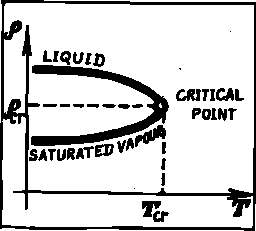
\includegraphics[width=0.5\textwidth]{figures/fig-04-03.pdf}
\caption{The critical point.}
\label{fig-4.3}
\end{figure}

If we compress a gas whose temperature is below criti­cal, the process of its compression can be depicted by an arrow intersecting the boiling point curve (\figr{fig-4.4}). This implies that at the moment of attaining a pressure equal to the vapour pressure (the point of intersection of the arrow with the boiling point curve), the gas starts condensing into a liquid. If our vessel were transparent, then at this moment we would see a layer of liquid forming at the bottom of the vessel. If the pressure does not change, the layer of liquid will grow until all of the gas has finally been transformed into the liquid. A further compression will now require an increase in pressure.
\begin{figure}[!ht]
\centering
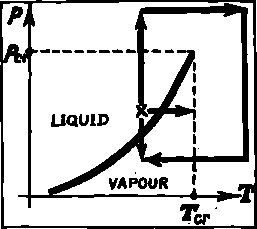
\includegraphics[width=0.5\textwidth]{figures/fig-04-04.pdf}
\caption{Implication of critical point in liquefaction of a gas.}
\label{fig-4.4}
\end{figure}
The situation is entirely different for the compression of a gas whose temperature is above critical. The process of compression can again be still depicted in the form of an arrow going upwards. But now this arrow does not intersect the boiling point curve. Hence, during the com­pression the vapour will not condense, but will only con­tinually become denser.

The existence of a gas-liquid interface is impossible at a temperature above critical. When compressed to arbi­trary densities, a uniform substance will be found under the piston, and it is hard to say when one may call it a gas and when a liquid.

The presence of the critical point shows that there is no difference in principle between the liquid and gaseous states. At first sight, it might seem that there is no such difference in principle only in case we are dealing with temperatures above critical. This, however, is not so. The existence of the critical point indicates the possi­bility of transforming a liquid, a genuine liquid, which can be poured into a glass, into the gaseous state avoiding the boiling process.

The path of such a transformation is shown in \figr{fig-4.4}. An unquestionable liquid is marked by a cross. If we lower the pressure somewhat (arrow pointing downwards), it will boil; it will also boil in case we raise the tempera­ture somewhat (arrow pointing to the right). But let us choose a different way. Let us compress the liquid so hard that its pressure exceeds critical. The point repre­senting the state of the liquid will rise vertically. Then let us heat the liquid -- this process will be depicted by a horizontal line. Now, after we have found ourselves to the right of the critical temperature, let us lower the pressure to its initial value. If we now decrease the tem­perature, we can obtain a most genuine vapour which could have been obtained from this liquid along a simpler and shorter path.

Therefore, by changing the pressure and temperature so that the critical point is avoided, it is always possible to obtain a vapour by means of a continuous transition from a liquid and vice versa. Such a continuous transition does not require boiling or condensation.

Early attempts to liquefy such gases as oxygen, nitro­gen and hydrogen were unsuccessful because the existence of the critical temperature was unknown. These gases have very low critical temperatures: \SI{-119}{\celsius} for oxygen, \SI{-147}{\celsius} for nitrogen and \SI{-240}{\celsius} or \SI{33}{\kelvin} for hydrogen. The record holder is helium, whose critical temperature is equal to \SI{4.3}{\kelvin}. It is possible to transform these gases to the liquid phase in only one way: we must lower their temperatures below the indicated values.

\section{Obtaining Low Temperatures}

A significant decrease in temperature can be attained by various means. But the idea involved in all these meth­ods is one and the same: we must force the body we want to cool to expend its internal energy.

But how can this be done? One of the ways is to make the liquid boil, not bringing in any heat from without. For this, as we know, it is necessary to decrease the pres­sure -- to reduce it to the value of the vapour pressure. The heat expended on the boiling will be taken from the liquid, and hence the temperature of the liquid and va­pour will fall; therefore, so will the vapour pressure. Consequently, in order that the boiling not cease but proceed more rapidly, it is necessary to continually pump air out of the vessel with the liquid.

However, a limit is reached to the fall in temperature during this process: the vapour pressure will eventually become completely negligible, and so even the most pow­erful pumps will be unable to create the required pres­sure.

In order to continue the lowering of temperature, we can, by cooling a gas with the aid of the liquid already obtained, convert it into a liquid with a lower boiling point. It is now possible to repeat the pumping process with the second substance and in this way to obtain lower temperatures. In case of necessity, such a cascade method of obtaining low temperatures can be extended.

Precisely in such a manner was this problem dealt with at the end of the past century, the liquefaction of gases was carried out in stages: ethylene, oxygen, ni­trogen and hydrogen, substances with boiling points of \SI{-103}{\celsius}, \SI{-183}{\celsius}, \SI{-196}{\celsius} and \SI{-253}{\celsius}, were successively converted into liquids. Having liquid hydrogen available, one can also obtain the lowest boiling liquid-helium (\SI{-269}{\celsius}). The neighbour ``to the left'' helped obtain the neighbour ``to the right''.

The cascade method of cooling is about a hundred years old. Liquid air was obtained by this method in 1877. Liquid hydrogen was first obtained in 1884-1885. Finally, the last stronghold was taken after another twenty years: helium, the substance with the lowest critical tempera­ture, was converted into a liquid in 1908 by Heike Kamerlingh Onnes (1853-1926) in Leiden, Holland. The 70th anniversary of this important scientific achievement was widely celebrated.

For many years, the Leiden laboratory was the only ``low-tempe-rature'' laboratory. But now there exist tens of such laboratories in many countries, not to mention the factories producing liquid air, nitrogen, oxygen and he­lium for technical purposes.

The cascade method of obtaining low temperatures is now rarely applied. In technical installations for lowering temperatures, a different means of decreasing the internal energy of a gas is applied: the gas is forced to expand ra­pidly and perform work at the expense of its internal energy.

If, for example, air is compressed up to several atmo­spheres and let into an expander, then when it performs the work involved in displacing a piston or rotating a turbine, it will cool off so abruptly that it liquefies. If carbon dioxide is let out of a cylinder with great speed, it will cool off so abruptly that it is converted into ``ice'' in the air.

Liquid gases have found wide application in technology. Liquid oxygen is used for explosives and as a component of the fuel mixture in jet engines.

The liquefaction of air is used in technology for sepa­rating the gases constituting air.
The temperature of liquid air is widely used in various branches of technology. But this temperature isn’t low enough for many physical investigations. In fact, if we convert the relevant temperatures expressed on the cen­tigrade scale to their values on the Kelvin scale, we shall see that the temperature of liquid air is approximately one-third of room temperature. Much more interesting for physics are ``hydrogen'' temperatures, i.e. temperatures of the order of 14-20 \si{\kelvin}, and especially ``helium'' tem­peratures. The lowest temperature obtained by pumping out liquid helium is \SI{0.7}{\kelvin}.

Physicists have succeeded in coming much closer to absolute zero. At the present time, temperatures have been obtained which are only several thousandths of a degree above absolute zero. However, these extremely low temperatures are obtained by methods which do not resemble those described above.

In recent years, cryogenics, the physics of low tem­peratures, has created the need leading to the founding of a new branch of industry. This branch is engaged in the manufacture of equipment and apparatus enabling large volumes and long conductors to be held at temperatures close to absolute zero.

\section{Supercooled Vapours and Superheated Liquids}

In passing through the boiling points, a vapour ought to condense, be transformed into a liquid. However, it turns out that if a vapour is very pure and does not come in contact with a liquid, we are able to obtain it in the form of a supercooled or supersaturated vapour -- a vapour which should have already become a liquid a long time ago.
A supersaturated vapour is very unstable. Sometimes it is sufficient to shake the vessel containing the vapour or throw a couple of grains into it for the delayed con­densation to immediately begin.

Experience shows that the condensation of steam mole­cules is greatly eased by the introduction of small alien particles. The supersaturation of water vapour does not occur in dusty air. It is possible to bring about conden­sation with puffs of smoke, since smoke consists of tiny solid particles. When the particles enter the steam, they gather molecules around themselves and become centres of condensation.

Thus, even though unstable, a vapour can exist in the region of temperatures fit for liquid ``life''.

But can a liquid ``live'' in the region of a vapour under those same conditions? In other words, is it possible to superheat a liquid?

It turns out to be possible. For this it is necessary to prevent the molecules of the liquid from breaking away from its surface. A radical means of achieving this is liquidating the free surface, i.e. placing the liquid in a vessel where it would be compressed on all sides by solid walls. Liquids have been successfully superheated in this manner by several degrees, i.e. one is able to displace a point depicting the state of a liquid to the right of its boiling point curve (see \figr{fig-4.4}).

Superheating is the displacement of a liquid into the region of a vapour; therefore, the superheating of a liquid can be achieved by lowering the pressure, as well as by supplying heat.

The former method can be used to obtain a surprising result. Water or some other liquid thoroughly freed of dissolved gases, which is not easy to do, is placed in a vessel with a piston reaching the surface of the liquid. The vessel and the piston should be wet by the liquid.

If we now draw the piston towards ourselves, the water cohering to the bottom of the piston will move along with it. But the layer of water cohering to the piston will pull the next layer of water after it, this layer will pull the one lying below it. As a result, the liquid will stretch.

The column of water will finally break (it is precisely the column that will break, but the water will not break away from the piston), but this will occur when the force on a unit of area attains tens of kilograms. In other words, a negative pressure of tens of atmospheres is created in the liquid.

The vapour phase of a substance is stable even for small positive pressures. And a liquid can be made to have a negative pressure. You couldn’t think of a more striking example of ``superheating''.

\section{Melting}
There is no solid body which would withstand a continual rise in temperature. Sooner or later a solid piece is transformed into a liquid; true, in certain cases we will not succeed in reaching the melting point -- a chem­ical decomposition may take place.
Molecules move more intensively as the temperature increases. Finally, the moment arrives when the preservation of order among the wildly ``swinging'' mole­cules becomes impossible. The solid body melts. Tungsten has the highest melting point: \SI{3380}{\celsius}. Iron melts at \SI{1539}{\celsius}, gold at \SI{1063}{\celsius}. Incidentally, there are also easily melted metals. Mercury, as is well known, will even melt at a temperature of \SI{-39}{\celsius}. Organic substances do not have high melting points. Naphthalene melts at \SI{80}{\celsius}, toluene at \SI{-94.5}{\celsius}.
 
It is not at all difficult to measure the melting point of a body, especially if it melts within the interval of temperatures which can be measured by an ordinary ther­mometer. It is completely unnecessary to keep one’s eye on the melting body. It is sufficient to look at the mercury column of the thermometer. The temperature of the body increases until the melting begins (\figr{fig-4.5}). As soon as the melting begins, the rise in temperature
ceases, and the temperature remains constant until the process of melting is completely finished.
\begin{figure}[!ht]
\centering
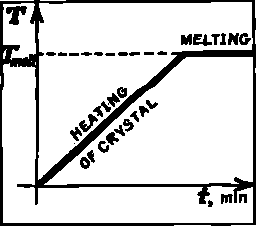
\includegraphics[width=0.5\textwidth]{figures/fig-04-05.pdf}
\caption{Finding melting point of a solid.}
\label{fig-4.5}
\end{figure}
Just as in the conversion of a liquid into a vapour, the conversion of a solid into a liquid requires heat. The amount of heat needed for this is called the \emph{latent heat of fusion}. For example, the melting of one kilogram of ice requires \SI{80}{\kilo\calorie}.

Ice is one of the bodies possessing a large heat of fusion. The melting of ice requires, for example, more than ten times as much energy as the melting of the same mass of lead. Of course, we are talking about the melting proper; here we are not dealing with the fact that before lead begins to melt, it must be heated up to \SI{+327}{\celsius}. The thawing of snow is delayed as a result of the large heat of fusion of ice. Imagine that its heat of fusion were ten times smaller. Then the spring thaws would lead each year to inconceivable disasters.

Thus, the heat of fusion of ice is great, but it is also small if we compare it with the heat of vaporization -- \SI{540}{\kilo\calorie\per\kilo\gram} (about seven times as small). This difference, by the way, is completely natural. Converting a liquid into a vapour, we must tear its molecules away from each other, but in melting a solid, we only have to destroy the order in the distribution of the molecules, leaving them almost at the same distances from each other. It is clear that less work is required in the latter case.

The possession of a definite melting point is an important feature of crystalline substances. It is on the basis of precisely this property that they are easily distinguished from other solids, called amorphous bodies or glasses. Glasses are found among organic substances as well as among inorganic ones. Window glass is usually made out of silicates of sodium and calcium; an organic glass (it is also called Plexiglas) is often placed on a desk.

In contrast to crystals, amorphous substances do not have a definite melting point. Glass does not melt, but softens. When heated, a piece of hard glass becomes soft, so that it can be easily bent or stretched; it begins to change its form at a higher temperature under the influence of its own weight. As it is further heated, the thick viscous mass of glass assumes the form of the vessel in which it is lying. This mass is at first as thick as honey, then as sour cream and, finally, becomes almost like a liquid with a small viscosity, such as water. With the best will in the world, here we are unable to single out a definite temperature at which the solid entered the liquid phase. The reasons for this lie in the radical differ­ence between the structure of glass and that of crystalline bodies. As has been said above, the atoms in amor­phous bodies are distributed disorderly. The structure of glass resembles that of a liquid. The molecules in hard glass are already distributed disorderly. Hence, a rise in the temperature of glass merely increases the amplitude of the oscillations of its molecules, gradually giving them more and more freedom of movement. Therefore, glass softens gradually and does not display the sharp transition from ``solid'' to ``liquid'', which is char­acteristic of a transition from the distribution of mole­cules in a strict order to their disordered distribution.

When discussing a boiling point curve, we said that a liquid and a vapour can exist, although in an unstable state, in alien regions -- a vapour can be supercooled and moved to the left of the boiling point curve, while a liq­uid can be superheated and drawn off to the right of the boiling point curve.

Are the analogous phenomena with respect to a crystal and a liquid possible? It turns out that the analogy here is incomplete.

If a crystal is heated, it will begin melting at its melting point. We shall not succeed in superheating a crystal. On the contrary, in cooling a liquid, we can, if we take certain steps, ``slip past'' the melting point with compa­rative ease. We are able to achieve considerable supercool­ings of certain liquids. There are even such liquids which are easy to supercool, but hard to make them crystallize. As such a liquid is cooled, it becomes more and more vis­cous and finally hardens without having crystallized. Glass is like that.

It is also possible to supercool water. Drops of mist can fail to freeze even during the most severe frosts. If a crystal of a substance (priming) is thrown into a super­ cooled liquid, then crystallization will immediately begin.

Finally, in many cases a delayed crystallization can begin as a result of shaking or other random events. It is known, for example, that crystalline glycerine was first obtained while being transported by train. After lying around for a long time, glass can begin to crystallize (devitrify).

\section{How to Grow a Crystal}

Under definite known conditions, crystals can be grown from almost any substance. Crystals can be obtained from a solution or from a melt of the given substance, as well as from its vapour (black rhombic crystals of iodine, for instance, are readily deposited from iodine vapour at standard pressure without an intermediate conversion into the liquid state).

Start by dissolving common salt or sugar in water. At room temperature (\SI{20}{\celsius}), you can dissolve up to \SI{70}{\gram} of salt in a thick glass (holding about \SI{200}{\gram} of water). If you keep adding salt, it will not dissolve, but will settle to the bottom in the form of a residue. A solution that can dissolve no more solute (as it is called) is said to be saturated with the given substance. If we change the temperature, the solubility of the solute in the solvent is changed as well. Everyone knows that hot water dissolves most substances more readily than cold water.

Imagine now that you have prepared a saturated solu­tion, say, of sugar, at a temperature of \SI{30}{\celsius} and cool it to \SI{20}{\celsius}. At \SI{30}{\celsius}, you can dissolve \SI{223}{\gram} of sugar in \SI{100}{\gram} of water, and at \SI{20}{\celsius}, only \SI{205}{\gram}. Then, in cooling from 30 to \SI{20}{\celsius}, \SI{18}{\gram} of sugar turn out to be ``redundant'' and, as they say, are precipitated from the solution. Hence, one of the possible ways to obtain crystals is to cool a saturated solution.

We can accomplish the same in a different way. Pre­pare a saturated solution of salt and let it stand in an open glass. After some time has passed you will find crystals of salt at the bottom. Why did they form? Look at the glass again, more carefully, and you can see that another change occurred together with the appearance of crystals: there is less water. The water evaporated and left ``redundant'' matter in the solution. Thus, still an­ other way to form crystals is to evaporate the solution.

How are crystals formed from a solution?

We mentioned that the crystals precipitate from the solution. Does this mean that no crystal was observed for a whole week and then, in a flash, it appears as if by magic? No, this is not so; crystals grow. You cannot, of course, observe the initial instant of growth with the naked eye. First, a few of the randomly moving mole­cules or atoms of the solute assemble by chance in approx­imately the same order required to form the crystal lattice. Such a group of atoms or molecules is called a \emph{nucleus}.

Experiments show that nuclei are more frequently formed when the solution contains extremely fine par­ticles, dust specks, of some foreign substance. Crystalli­zation proceeds at the highest rate and most easily if a tiny seed crystal is put into the saturated solution. Then the precipitation of the solid substance from the solution consists in the growth of the seed crystal rather than in the formation of new small crystals, i.e. in nucleation.

The growth of a nucleus does not, of course, differ in any way from the growth of a seed crystal. The advantage of using a seed crystal is that it ``draws'' to itself the sub­ stance separating out of the solution, hindering, in this way, the formation of a large number of nuclei. If a great many nuclei are formed at once, they impede each other in growing and we cannot obtain large crystals.

How do new portions of atoms or molecules, separating out of the solution, arrange themselves on the surfaces of the nucleus?

It has been found that the growth of a nucleus or seed crystal consists in the seemingly outward motion of its faces in a direction perpendicular to each face so that they remain parallel to their initial positions (the crys­tal seems to expand). Naturally, the angles between the faces remain constant (we already know that the con­stancy of these angles is one of the vital features of crys­tals and is due to their lattice structure).
\begin{figure}[!ht]
\centering
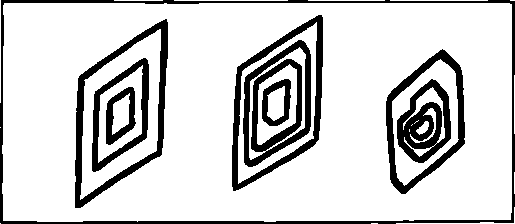
\includegraphics[width=\textwidth]{figures/fig-04-06.pdf}
\caption{Modes of crystal growth.}
\label{fig-4.6}
\end{figure}
The successive outlines during the growth of three differ­ent crystals of the same substance are shown in \figr{fig-4.6}. Similar pictures can be observed in a microscope. For the crystal shown at the left the number of faces remains constant during the growth. The middle crystal is an example of how a new face appears during the growth (at the upper right) and subsequently disappears.

It is important to note that the rate of growth of the faces, i.e. the velocity at which the faces seem to move while remaining parallel to their initial positions, is not the same for various faces. We also find that the faces that disappear are those that grow fastest, for instance, the lower left face in the middle crystal. The slowest-growing faces, on the contrary, become the videst or, as we say, best-developed, ones. It is a principle that a grown crystal is always bounded by its slowest-growing faces.

This is especially clear from the illustration at the right in \figr{fig-4.6}. Here a formless fragment acquires the same shape as the other crystals precisely owing to the anisotropy of growth rates. Quite definite faces devel­op at the expense of others more and more resolutely, and impart the shape, or habit, to the crystal that is inherent in all specimens of this substance.

Very handsome intermediate shapes are observed if a sphere is taken as a seed crystal and the solution is alternately cooled slightly and then heated slightly. Upon being heated the solution becomes undersaturated and the seed crystal is partly dissolved. Cooling leads to oversaturation of the solution and growth of the seed crystal. But the molecules attach themselves differently than they were before being dissolved, seeming to give preference to certain locations. The substance is thus transferred from certain parts of the sphere to other parts. First small circular faces appear on the surface of the sphere. These circles gradually increase in size and, contacting one another, merge along straight edges. The sphere is converted into a polyhedron. Then certain faces overtake others in their growth, a part of the faces become smaller and smaller and disappear. 
\begin{figure}[!ht]
\centering
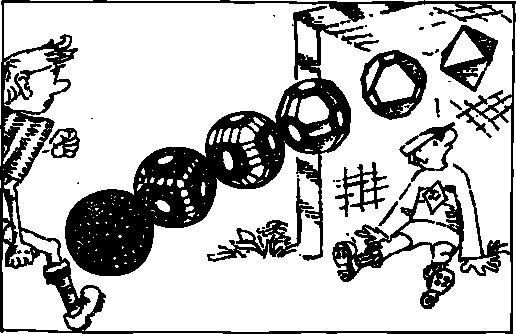
\includegraphics[width=\textwidth]{figures/fig-04-07.pdf}
\caption{Attaining the characteristic shape of a crystal by growing from a sphere as a seed crystal.}
\label{fig-4.7}
\end{figure}
Finally, the crystal reaches its characteristic shape, or habit (\figr{fig-4.7}). In observing the growth of a crystal, one of its features may astound us -- the seemingly parallel motion of its faces. This implies that the substance separating out of the solution is deposited on the faces in layers, and that a succeeding layer is not started until the preceding one
is completed.

Illustrated in \figr{fig-4.8} is an ``incompleted'' packing arrangement of atoms. In which of the positions indicated by letters is a new atom, attaching itself to the crystal, most likely to remain secured? Without doubt, in posi­tion $K$ because here it is subject to attraction by its neigh­bours from three sides. In position $L$ the new atom is attracted from two sides, and in position $M$ from only one. This is why a row is first completed, then a whole layer and finally a new layer is started.
\begin{figure}[!ht]
\centering
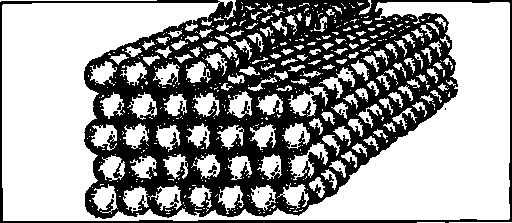
\includegraphics[width=\textwidth]{figures/fig-04-08.pdf}
\caption{An ``incompleted'' packing arrangement of atoms..}
\label{fig-4.8}
\end{figure}
In many cases, crystals are formed from a molten mass, or melt. This takes place on an immense scale in nature; basalts, granites and other kinds of igneous rocks were formed of fiery magma.

Let us heat some kind of crystalline substance, for example, rock salt. Up to a temperature of \SI{804}{\celsius}, the salt crystals change very slightly; they only expand negligibly, but the substance remains a solid. A thermom­eter placed in the vessel with the substance indicates a continuous increase in temperature during heating. At \SI{804}{\celsius}, we discover two new interrelated phenomena: the substance begins to melt and the temperature ceases to increase any further. Until all of the substance is con­verted into a liquid, the temperature remains unchanged. A further increase in temperature indicates that we are heating the liquid. All crystalline substances have a def­inite melting point. Ice melts at \SI{0}{\celsius}, iron at \SI{1527}{\celsius} and mercury at \SI{39}{\celsius} below zero, etc.

As we already know, in each small crystal the atoms or molecules of the substance form an ordered packing arrange­ment and have small vibrations about their mean posi­tions. As the body is heated, the velocity of the vibrating particles increases together with the amplitude. This increase in the velocity of motion of particles as the tem­perature is raised is one of the basic laws of nature and concerns matter in any state -- solid, liquid or gaseous.

When the temperature of the crystal has reached a definite, sufficiently high value, the vibration of its particles becomes so violent that an accurate arrangement of the particles is no longer possible; the crystal melts. As melting begins, the heat supplied no longer increases the velocity of motion of the particles, it is employed to break up the crystal lattice. This is why the temperature remains constant until all of the substance melts. Subsequent heating increases the velocity of the particles of liquid.

In our case of crystallization from a melt, called freez­ing, all the phenomena described above occur in the reverse order: as the liquid is cooled, the chaotic motion of its particles slows down. When a definite, sufficiently low temperature has been reached, the velocity of the particles is so low that some of them begin to align themselves with others, forming a crystal nucleus. Until the whole substance has frozen, or solidified, the temperature remains constant. As a rule, this temperature is the same as the melting point.

Unless special measures are taken, freezing begins in the melt simultaneously at many places. The small crystals begin to grow as regular polyhedrons character­istic of the given substance in exactly the same way as we described above. Such free growth soon ends, however, because the growing small crystals run into one another, with further growth ceasing at the points of contact. This imparts a granular structure to the solidified body. Each grain is a small crystal that was unable to assume its regular shape.

Depending on many factors, and primarily on the cooling rate, a solid can consist of coarser or finer grains. The lower the cooling rate, the coarser the grains. The grain size of crystalline bodies ranges from a millionth of a centimetre to several millimetres. In the majority of cases, the granular crystalline structure can be observed under a microscope. Most solids have such a fine- crystalline structure.

The freezing of metals is a process of vital interest to engineering. Physicists have investigated in exceptionally great detail the phenomena occurring when molten metal is poured into a mould in a foundry and solidifies.

Mostly small tree-like crystals, called \emph{dendrites}, grow in a molten metal when it is cooled. Sometimes the dendrites are oriented at random, and sometimes they are parallel to one another.
\begin{figure}[!ht]
\centering
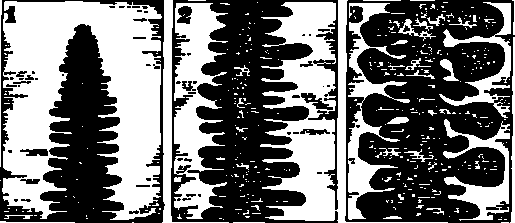
\includegraphics[width=\textwidth]{figures/fig-04-09.pdf}
\caption{Stages of growth of single dendrite.}
\label{fig-4.9}
\end{figure}
The stages of growth of a single dendrite are illustrated in \figr{fig-4.9}. Under such circumstances, the dendrite can become overgrown, occupying all the space between its branches, before encountering another dendrite in the melt. Then we find no dendrites in the solidified casting. But events can develop differently: dendrites may meet and grow into one another (with the branches of one filling the spaces between the branches of another) while they are still in an early stage of growth.

Hence, we may obtain castings whose grains (shown in \figr{fig-2.22}) have very different structures. The properties of metals depend essentially upon this structure. We can control the behaviour of a metal in solidifying by varying the cooling rate and the system of heat dis­posal from the mould.

If we wish to grow a large single crystal, we must take steps to have the crystal grow in one place. But if several crystals have already started growing, then in any case we must take steps to make the conditions for growth favourable for only one of them.

Here, for example, is what one does in growing crystals of fusible metals. The metal is melted in a glass test tube with a drawn-out bottom. The test tube, suspended on a thread inside a vertical cylindrical oven, is slowly low­ered. The drawn-out bottom gradually leaves the oven and cools off. Crystallization begins. At first, several tiny crystals are formed, but those which grow sideways come up against the test tube wall and their growth is slowed down. Only the crystal which grows along the axis of the test tube, i.e. into the heart of the melt, proves to be in favourable conditions. As the test tube is lowered, new portions of the melt coming into a low-temperature region will ``feed'' this unique crystal. Therefore, of all the tiny crystals, it alone will survive; as the test tube is lowered, it continues to grow along its axis. At last, all of the melted metal hardens in the form of a single crystal.

The same idea underlies the growing of refractory crys­tals of ruby. Fine ruby powder is poured in a stream through a flame. As a result, the particles of powder melt; tiny droplets fall on a refractory support of very small area forming a mass of crystals. 

During the further fall of droplets on the support, all the tiny crystals will grow, but once again only the one which is in the most advantageous position for ``receiving'' the falling drops will de­velop.

But what are large crystals needed for?

Industry and science are often in need of large single crystals. Of great significance for technology are crystals of Seignette salt and quartz possessing the remarkable property of transforming mechanical action (for example, pressure) into voltage.

The optical industry needs large crystals of calcite, rock salt, fluorite, etc.

Crystals of ruby, sapphire and certain other precious stones are needed for the watchmaking. The reason for this is that individual movable parts of ordinary watches perform up to \num{20000} oscillations per hour. This makes unusually heavy demands on the quality of the tips of the axes and the bearings. The wear will be least when ruby or sapphire serves as the bearing for the tip of an axis of 0.07-0.15 \si{\milli\meter} in diameter. 

Artificial crystals of these substances are very durable and are worn out very little by steel. It is remarkable that artificial stones prove to be better for this purpose than the same natural stones.

Of greatest significance in industry, however, is the growing of semiconductor (silicon) monocrystals. The communications-electronics of today is inconceivable without these crystals.

\section{Influence of Pressure on Melting Point}

If the pressure is changed, the melting point will also change. We came across such a regularity when dealing with boiling. The greater the pressure, the higher the boiling point. As a rule, this is also true for melting. However, there are a small number of substances which behave anomalously: their melting points decrease with an increase in pressure.

The fact of the matter is that the vast majority of solids are denser than their liquids. The exceptions to this rule are precisely those substances whose melting points change somewhat unusually with a change in pressure, for example, water. Ice is lighter than water, and the melting point of ice is lowered by an increase in pressure.

Compression facilitates the formation of the denser state. If the solid is denser than the liquid, then compres­sion aids solidification and hinders melting. But if melting is obstructed by compression, this means that the substance remains solid, whereas previously it would have melted at this temperature, i.e. the melting point rises with an increase in pressure. In an anomalous case, the liquid is denser than the solid, and so the pressure helps to form the liquid, i.e. lowers the melting point.

The influence of the pressure on the melting point is much less than the analogous effect for boiling. An increase in pressure of more than \SI{100}{\kgf\per\centi\meter\squared} lowers the melting point of ice by \SI{1}{\celsius}.

Why is it that skates glide on ice but do not slide on a highly polished parquet floor that is just as smooth as ice? The only feasible explanation, evidently, is the formation of water which lubricates the runners of the skates. But the pressure exerted by the runner does not in any case exceed \SI{100}{\kgf\per\centi\meter\squared}, and this would not seem to lower the melt­ing point of the ice sufficiently so that it melts under the runners. All I can say to eliminate this contradiction is the following: skates with blunt runners slide very poorly on ice. The runners must be ground so that they cut the ice. Then only the sharp edges of the runners contact the ice, exerting a pressure of tens of thousands of atmospheres and the ice \emph{does} melt.

\section{Evaporation of Solids}

When we say that a substance is evaporating, it is usually implied that a liquid is evaporating. But solids can also evaporate. The evaporation of solids is sometimes caed \emph{sublimation}.

Naphthalene, for example, is an evaporating solid. Naphthalene melts at \SI{80}{\celsius}, but evaporates at room tem­perature. It is precisely this property of naphthalene which enables it to be used for the extermination of moths. A fur coat powdered with naphthalene will become saturated with naphthalene vapours, creating an atmo­sphere which moths cannot bear. Every solid with an odour sublimes to a significant degree. In fact, the odour is created by the molecules which have broken away from the substance and reached our nose. However, the cases where a substance sublimes to an insignificant degree, sometimes to a degree that cannot be detected by even the most careful investigation, are more frequent. In prin­ciple, any solid (yes, any, even iron or copper) evaporates. If we do not detect sublimation, this merely means that the saturated vapour density is very negligible.
\begin{figure}[!ht]
\centering
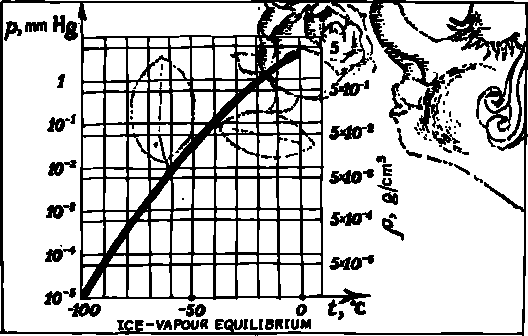
\includegraphics[width=\textwidth]{figures/fig-04-10.pdf}
\caption{Saturated vapour density as a function of temperature.}
\label{fig-4.10}
\end{figure}
The saturated vapour density in equilibrium with the solid grows rapidly with temperature (\figr{fig-4.10}). It is possible to convince oneself that a number of substances having sharp odours at room temperature lose them at low temperatures.

In most cases it is impossible to considerably increase the saturated vapour density of a solid for a simple rea­son -- the substance will melt beforehand.

Ice also evaporates. This is well known to housewives who hang up their wash to dry during a frost. At first the water will freeze, but then the ice evaporates and the wash turns out to be dry.


\section{Triple Point}

Thus, there are conditions under which a vapour, a liquid and a crystal can exist pairwise in equilibrium.

Can all three states be in equilibrium? Such a point exists on the pressure-temperature diagram, it is called the \emph{triple point}. Where is it located?

If ice floating on water is placed in a closed vessel at a temperature of zero degrees, water (and ``ice'') vapour will start entering the free space. At a pressure of \SI{4.6}{\milli\meter\mercury}, evaporation will cease and saturation will set in. Now the three phases, ice, water and vapour, will be in a state of equilibrium. This is precisely the triple point.

\begin{figure}[!ht]
\centering
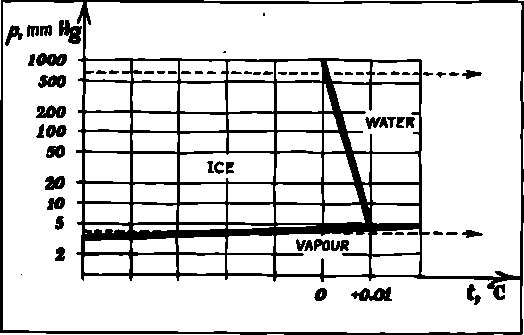
\includegraphics[width=\textwidth]{figures/fig-04-11.pdf}
\caption{Relationship between various states (phases) of water showing the triple point.}
\label{fig-4.11}
\end{figure}
The relationships between the various states are graph­ically and clearly shown by the diagram for water depict­ed in \figr{fig-4.11}. Such a diagram can be constructed for any substance.

We are acquainted with the curves in the diagram -- they are the equilibrium curves for ice and water vapour, ice and water, and water and water vapour. As is customary, the pressure is plotted along the vertical axis, and the temperature along the horizontal.

The three curves intersect in the triple point and divide the diagram into three regions -- the living spaces for ice, water and water vapour.

Phase diagram is a concise handbook. Its aim is to answer questions as to what state of a substance is stable at a given pressure and a given temperature.

If water or water vapour is placed under the conditions of the ``left-hand region'', it will turn into ice. If water or ice is introduced into the ``lower region'', water vapour will be obtained. In the ``right-hand region'', water va­pour will condense and ice will melt.

The phase diagram permits one to immediately say what will happen to a substance when it is heated or compressed. Heating at a constant pressure will be depicted on the diagram by a horizontal line. The point depicting the phase of the substance will move from left to right along this line.

Two such lines are depicted in the figure, one of which is heating under standard pressure. This line lies above the triple point. Therefore, it will first intersect the melting point curve, and then, beyond the bounds of the diagram, the evaporation curve too. Under standard pressure, ice melts at a temperature of \SI{0}{\celsius}, while the water so formed will boil at \SI{100}{\celsius}.

The situation will be different for ice heated under a very low pressure, say, a bit less than 5 mm Hg. The heating process is depicted by a line passing beneath the triple point. The melting and boiling point curves do not intersect this line. Under such a negligible pressure, heating leads to a direct transition of ice to water vapour.

\begin{figure}[!ht]
\centering
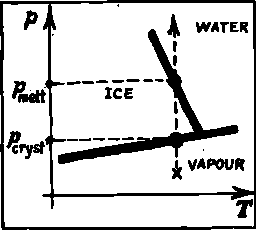
\includegraphics[width=0.5\textwidth]{figures/fig-04-12.pdf}
\caption{Phase digram can be used for predicting what happens at particular pressure and temperature.}
\label{fig-4.12}
\end{figure}
In \figr{fig-4.12}, this same diagram shows what an inter­esting phenomenon will occur when water vapour in the state marked on the figure by a cross is compressed. The vapour will first be converted into ice, which will then melt. The diagram enables us to say at once at what pressure the growth of crystals will begin and when the melting takes place.

The phase diagrams for all substances resemble each other. Significant, from the everyday point of view, differ­ences arise because the location of the triple point on the diagram can be most diverse for various substances.

After all, we exist under conditions which are close to ``standard'', i.e. in the first place, under a pressure close to one atmosphere. The way in which the triple point of a substance is located with respect to the standard pressure line is very important for us.
If the pressure at the triple point is less than atmospher­ic, then for us, living under ``standard'' conditions, the substance will be one of those that melt. As the temper­ature rises, it will first be transformed into a liquid, which will then boil.

In the opposite case, when the pressure at the triple point is higher than atmospheric, we will not see any liquid when the substance is heated, since the solid will be converted directly into a vapour. This is how ``dry ice'' behaves, which is very convenient for ice cream vendors.

They can distribute pieces of ``dry ice'' among the portions of ice cream without worrying that the ice cream will become wet as a result. “Dry ice” is solid carbon dioxide, \ce{CO2}. Its triple point lies at \SI{73}{\atmos}. Therefore, when solid \ce{CO2} is heated, the point depicting its state will move along a horizontal line intersecting only the evaporation curve of the solid (just as for ordinary ice at a pressure of about \SI{5}{\milli\meter\mercury}).

We have already explained how one degree of temper­ature on the Kelvin scale, or kelvin (as we are now required to call it by the SI system), is determined. The point of the discussion there was the principle involved in determining temperatures. But not all metrological institutes have ideal gas thermometers at their disposal. Therefore, a temperature scale is usually established with the aid of points of equilibrium, fixed by nature, between various states of substances.

Of especial significance in this matter is the triple point of water. A kelvin is determined today as 1/273.16 of the thermodynamic temperature of the triple point of water\footnote{In the 2019 redefinition of SI units, the kelvin was changed completely. Now the kelvin is defined in terms of the energy equivalent as given by Boltzmann's equation, , the scale remains the same numerically, i.e. the triple point of water is still the same. -- Damitr}. The triple point of oxygen is taken equal to \SI{54.361}{\kelvin}. The freezing point of gold is equal to \SI{1337.58}{\kelvin}; Using these datum points we can readily graduate any ther­mometer.

\section{The Same Atoms but Different Crystals}

The dull, soft graphite with which we write and the bright, transparent, hard, cutting glass, diamond are made of one and the same atoms -- atoms of carbon. Why then are there such differences between the properties of these two substances identical in composition?
Recall the lattice of flaky graphite each of whose atoms has three nearest neighbours, and the lattice of diamond whose atoms have four nearest neighbours. It is clearly evident from this example how the properties of crystals are determined by the mutual distribution of their atoms. Fireproof crucibles, withstanding temperatures up to two or three thousand degrees, are made of graphite, but diamond burns at temperatures above \SI{700}{\celsius}; the spe­cific gravity of diamond is 3.5, of graphite 2.3; graphite conducts electricity, but diamond does not, etc.

This property of forming various crystals is possessed not only by carbon. Almost every chemical element, and not only element but also any chemical substance, can exist in several varieties. Six varieties of ice, nine varieties of sulphur and four varieties of iron are known.

In discussing a phase diagram, we did not speak of the various types of crystals, but drew a single region for the solid. But for a great many substances, this region is divided up into sections each of which corresponds to a definite ``sort'' of solid body or, as one says, a definite solid phase (a definite crystal modification).

Each crystal phase has its own region of stable state bounded by definite intervals of pressure and temperature. The laws of transformation of one crystal variety into another are the same as the laws of melting and evapora­tion.

Given any pressure, one can find a temperature at which both types of crystals will peacefully coexist. If we raise the temperature, a crystal of one form will be converted into a crystal of the second. If we lower the temperature, the reverse transformation will take place.

In order to convert red sulphur into yellow under stan­dard pressure, a temperature below \SI{110}{\celsius} is needed. Above this temperature, right up to the melting point, the order of the distribution of atoms characteristic of red sulphur is stable. When the temperature falls, the oscillations of the atoms decrease, and, beginning with \SI{110}{\celsius}, nature finds a more convenient order for the dis­tribution of the atoms. A transformation of one crystal into another occurs.

Nobody has thought of names for the six different ices. This is what one says: ice one, ice two, \ldots, ice seven. How come seven if there are only six varieties? The rea­son is that repeated experiments have failed to detect ice four.

If water is compressed at a temperature of about zero, ice five will be formed at a pressure of about \SI{2000}{\atmos}, and ice six at a pressure of about \SI{6000}{\atmos}.

Ice two and ice three are stable at temperatures below zero degrees centigrade.

Ice seven is a hot ice; it appears when hot water is sub­jected to a pressure of about \SI{20000}{\atmos}.

All ices, except the ordinary one, are heavier than water. Ice obtained under standard conditions behaves anoma­lously; on the contrary, ice obtained under conditions differing from the norm behaves normally.

We say that each crystal modification is characterized by a definite region of existence. But if so, how can graph­ite and diamond possibly exist under identical condi­tions?
Such ``lawlessness'' is found very often in the world of crystals. The ability to live under ``alien'' conditions is almost a rule for crystals. While one must turn to various tricks in order to transfer a vapour or a liquid to alien regions of existence, a crystal, on the contrary, can almost never be forced to stay within the frontiers marked off for it by nature.

The superheating and supercooling of crystals are explained by the difficulty in transforming one order into another under conditions of extreme overcrowding. Yel­low sulphur should be transformed into red at \SI{95.5}{\celsius}. During a more or less rapid heating, we ``slip past'' this transformation point and drive it up to \SI{113}{\celsius}.

The true transformation point is most easily detected when different crystals are in contact. If we put one up close against the other and maintain a temperature of \SI{96}{\celsius}, the yellow sulphur will be eaten up by the red, but the yellow will swallow the red at \SI{95}{\celsius}. Unlike a ``crystal-liquid'' transition, a ``crystal-crystal'' transfor­mation is ordinarily delayed during superheating, just as during supercooling.

In certain cases, we come across states of a substance which are supposed to exist at entirely different temper­atures.

White tin must turn into grey when the temperature falls to \SI{+13}{\celsius}. We ordinarily use things made of white tin and know that nothing will happen to them in winter. White tin withstands supercooling of 20-30 degrees per­fectly well. However, under conditions of a severe winter, white tin is transformed into grey. The lack of knowledge of this fact was one of the circumstances destroying Scott’s expedition to the South Pole (1912). The liquid fuel taken along by the expedition was kept in vessels soldered with tin. During severe frosts, the white tin was transformed into a grey powder, the vessels came unsoldered and the fuel was spilt. Not without reason is the appear­ance of grey spots on white tin called tin plague.

Just as in the case of sulphur, white tin can be converted into grey at a temperature a bit lower than \SI{13}{\celsius}, if a tiny grain of the grey variety falls on a tin object.

The existence of several varieties of one and the same substance and the delays in their mutual transformations have great significance for technology.

At room temperature, iron atoms form a body-centred cubic lattice, occupying the vertices and centre of each cube. Every atom has 8 neighbours. At a high tempera­ture, iron atoms form a denser ``packing'' -- each atom has 12 neighbours. Iron with 8 neighbours per atom is soft; iron with 12 neighbours per atom is hard. It turns out that it is possible to obtain iron of the latter type at room temperature. The method whereby this is done, hardening, is widely applied in metallurgy.

Hardening is accomplished quite simply -- the metallic object is made red-hot and then thrown into water or oil. Cooling occurs so rapidly that there is no time for the transformation of the structure stable at a high temper­ature to take place. Consequently, the high-temperature structure will exist indefinitely under conditions unnat­ural to it; recrystallization into a stable structure occurs so slowly that it is practically unnoticeable.

In speaking of the hardening of iron, we were not quite exact. Steel, i.e. iron containing a fraction of a percent of carbon, is hardened. The presence of very small admix­tures of carbon delays the transformation of hard iron into soft and permits the hardening to be carried out. As for completely pure iron, one cannot succeed in hardening it -- there is time for the conversion of its structure to take place even during the most rapid cooling.
Depending on the form of the phase diagram, one or another transformation is achieved by changing the pres­sure or the temperature.

Many transformations of a crystal into a crystal are observed during a change of only the pressure. Black phosphorus was obtained in this way.
\begin{figure}[!ht]
\centering
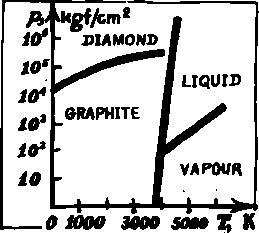
\includegraphics[width=0.5\textwidth]{figures/fig-04-13.pdf}
\caption{The phase diagram of carbon.}
\label{fig-4.13}
\end{figure}
Graphite was able to be converted into diamond only by simultaneously using both high temperature and pressure. The phase diagram for carbon is depicted in \figr{fig-4.13}. At pressures below ten thousand atmospheres and at tem­peratures less than \SI{4000}{\kelvin}, graphite is the stable modi­fication. Therefore, diamond exists under “alien” con­ditions, and so it can be transformed into graphite without particular difficulty. But the inverse problem is of prac­tical interest. We cannot succeed in carrying out a transformation of graphite into diamond by only raising the pressure. A phase transformation in the solid state apparently goes too slowly. The form of the phase diagram suggests the correct solution: increase the pressure and heat the graphite simultaneously. We then obtain upper
right-hand corner of the diagram) melted carbon. Cooling it at a high pressure, we should enter the region of dia­mond.

The practical possibility of such a process was proved in 1955, and at the present time the problem is considered to be solved from technological point of view.

\section{An Amazing Liquid}

If we lower the temperature of a body, sooner or later it will solidify and acquire a crystal structure. Moreover, it makes no difference at what pressure the cooling takes place. This circumstance seems perfectly natural and understandable from the point of view of the physical laws with which we have already become acquainted. In fact, by lowering the temperature, we decrease the intensity of the thermal motion. When the motion of molecules becomes so weak that it has already ceased to interfere with the forces of interaction between them, the molecules will line up in an accurate order -- will form crystals. A further cooling will take away from the mole­cules all the energy of their motion, and at absolute zero, a substance should exist in the form of molecules at rest distributed in a regular lattice.

Experiments show that all substances behave in this manner. All but one unique substance: this ``freak'' is helium. We have already informed the reader of certain facts concerning helium. It holds the record for the value of its critical temperature. Not a single substance has its crit­ical temperature lower than \SI{4.3}{\kelvin}. However, this record by itself does not imply anything amazing. Something else is startling: cooling helium below the critical tem­perature and practically reaching absolute zero, we will not obtain solid helium. Helium remains liquid even at absolute zero.

The behaviour of helium is completely unexplainable from the point of view of the laws of motion presented by us, and is one of the signs of the limited validity of the laws of nature which seemed universal.

If a substance is liquid, its atoms are in motion. But in cooling it down to absolute zero, we have taken all the energy of motion away from it. We have to admit that helium has an energy of motion which cannot be taken-away. This conclusion is incompatible with the mechan­ics which we have been studying so far. According to the mechanics we learned, the motion of a body can always be slowed down to a complete halt by taking away all its kinetic energy; the motion of molecules can also be stopped in exactly the same way by taking energy away from them during collisions with the walls of the vessel being cooled. Such a mechanics will obviously not do for helium.

The ``strange'' behaviour of helium is an indication of a fact of enormous importance. This is the first time that we have come up against the impossibility of applying in the world of atoms the basic laws of mechanics established by means of a direct investigation of the motion of visible bodies -- laws which seemed to constitute a firm founda­tion for physics.

The fact that helium ``refuses'' to crystallize at absolute zero is by no means possible to reconcile with the mechan­ics which we have been studying until now. The contradiction which we have come across for the first time, that atoms do not obey the laws of mechanics, is merely the first link in a chain of sharper and more glaring con­tradictions in physics.

These contradictions have led to the necessity of revis­ing the foundations of the mechanics of atomic motion. This revision is very profound and has led to a change in our entire understanding of nature.
\begin{figure}[!h]
\centering
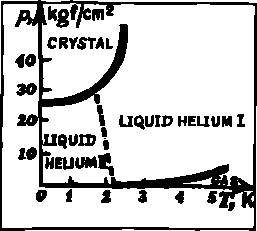
\includegraphics[width=0.5\textwidth]{figures/fig-04-14.pdf}
\caption{Phase diagram for Helium.}
\label{fig-4.14}
\end{figure}


The necessity for a radical revision of the mechanics of atomic motion does not imply that we must give up the laws of mechanics we have studied as a bad job. It would have been unfair to make the reader study unnecessary things. The old mechanics is completely valid in the world of large bodies. This is already enough for us to regard the corresponding chapters of physics with complete respect. However, it is also important that a number of laws of the ``old'' mechanics pass over without change into the ``new'' mechanics. Among them, in particular, is the law of conservation of energy.

The presence of ``inalienable'' energy at absolute zero is not a special property of helium. It turns out that all substances have ``zero'' energy. Only for helium does this energy prove sufficient to prevent the atoms from forming a regular crystal lattice.
One must not think that helium cannot occur in a crys­talline state. It is merely necessary to raise the pressure to approximately \SI{25}{\atmos} in order to crystallize helium. Cooling carried out above this pressure leads to the for­mation of solid crystalline helium with perfectly ordinary properties. Helium forms a face-centred cubic lattice.

The phase diagram for helium is shown in \figr{fig-4.14}. It differs greatly from the diagrams of all other sub­stances in the absence of a triple point. The melting and boiling point curves do not intersect.